\chapter{Træer}
\section{Terminologi for træer}

Sammenhængende grafer, der ikke indeholder en simpel kreds, kaldes træer. Træer har anvendelser i en del forskellige algoritmer.

\begin{defn}
Et træ er en sammenhængende ikke-orienteret graf, der ikke indeholder en simpel kreds.
\label{def_tree}
\end{defn}

\noindent Træer er en type af simple grafer. Da de ikke indeholder en simpel kreds, kan der ikke være flere kanter mellem to knuder, og der kan ikke være løkker. Alternativt og ekvivalent til Definition \ref{def_tree} kan et træ defineres som følger.

\begin{thm}
En ikke-orienteret graf er et træ hvis og kun hvis, der eksistrerer netop én simpel vej mellem hvert par af knuder. 
\end{thm}

\begin{proof}
Antag at en ikke-orienteret graf $T$ er et træ, og lad $u$ og $v$ være to knuder i $T$. 
Da $T$ er sammenhængende må det betyde, at der er en simpel vej mellem $u$ og $v$ jf. Sætning \ref{smh_satning}. 
Den simple vej mellem $u$ og $v$ må være den eneste vej mellem $u$ og $v$, for hvis der eksisterer flere veje mellem $u$ og $v$, eksisterer en simpel kreds. 
Hvis der mellem $u$ og $v$ er to forskellige simple veje $P_{u,v}$ og $P_{v,u}$, må der være mindst ét punkt, der er forskelligt mellem de to veje. 
En simpel kreds opstår fra og med knuden, hvor $P_{u,v}$ og $P_{v,u}$ første gang adskiller sig fra hinanden. 
Den simple kreds slutter, når $P_{u,v}$ og $P_{v,u}$ igen har en knude til fælles.
 Eksistensen af en simpel kreds modstrider antagelsen om, at $T$ er et træ, og derfor må der være netop én simpel vej mellem hvert knudepar i $T$.

Antag nu, at der er netop én simpel vej mellem hvert knudepar i en ikke-orienteret graf $T$. Det betyder, at $T$ er sammenhængende. Desuden må det gælde, at $T$ ingen simple kredse har, da det vil stride i mod antagelsen om, at der er netop én simpel vej mellem hvert knudepar i en $T$. Der kan ikke eksistere en simpel kreds, der kun er én simpel vej mellem to knuder $u$ og $v$, og derfor kan der ikke findes punkter, hvor to eller flere veje mellem $u$ og $v$ er forskellige fra hianden, hvor der kan dannes en kreds. Grafen $T$ opfylder dermed kravene for at være et træ jf. Definition \ref{def_tree}.
\end{proof}

\begin{exmp}
For at illustrere en graf, som er et træ, og en graf, som ikke er et træ, iagttages hhv. Figur \ref{eksempel_tree} og Figur \ref{eksempel_notree}. Grafen i Figur \ref{eksempel_tree} er et træ, da det er en ikke-orienteret sammenhængende graf uden simple kredse.
\end{exmp}

\begin{figure}[h]
\centering
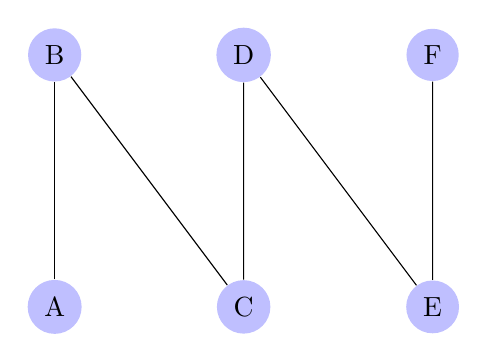
\begin{tikzpicture}
[scale=.8,auto=left,every node/.style={circle,fill=blue!25}]
  \node (n6) at (3,2) {A};
  \node (n4) at (3,6) {B};
  \node (n5) at (6,2) {C};
  \node (n1) at (6,6) {D};
  \node (n2) at (9,2) {E};
  \node (n3) at (9,6) {F};
  \foreach \from/\to in {n6/n4,n4/n5,n5/n1,n1/n2,n2/n3}
    \draw (\from) -- (\to);
\end{tikzpicture}
\caption{Et træ.} 
\label{eksempel_tree}
\end{figure}

\noindent Grafen i Figur \ref{eksempel_notree} er ikke et træ, da der eksistrer en kreds $\lbrace B, D, C \rbrace$. Grafen er heller ikke et træ med argumentet, at grafen ikke er sammenhængende.\\

\begin{figure}[h]
\centering
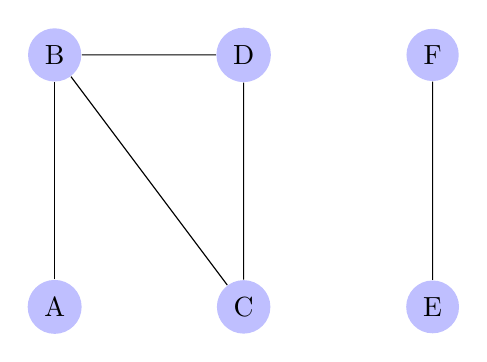
\begin{tikzpicture}
[scale=.8,auto=left,every node/.style={circle,fill=blue!25}]
  \node (n6) at (3,2) {A};
  \node (n4) at (3,6) {B};
  \node (n5) at (6,2) {C};
  \node (n1) at (6,6) {D};
  \node (n2) at (9,2) {E};
  \node (n3) at (9,6) {F};
  \foreach \from/\to in {n6/n4,n4/n5,n5/n1,n2/n3,n4/n1}
    \draw (\from) -- (\to);
\end{tikzpicture}
\caption{En graf, der ikke er et træ.} 
\label{eksempel_notree}
\end{figure}

\noindent Mange anvendelser af træer, kræver at en bestemt knude i en graf fungerer som udgangspunkt. En knude kan indentificeres som en rod, og dermed rodfæste grafen.

\begin{defn}
Et rodfæstet træ er et træ med en knude, der er udnævnt som roden. De resterende knuder er orienteret væk fra roden.
\end{defn}

\noindent Der findes terminologi, der beskriver knudernes forhold til hinanden i en rodfæstet graf. 
Hvis $T$ er et rodfæstet træ, så er en knude $v$, som ikke er roden, $\textit{forælder}$ til en knude $u$, hvis der eksiterer en orienteret kant fra $v$ til $u$ i retningen væk fra roden.
Samtidigt er $u$ $\textit{barn}$ af $v$, og knuder med samme forælder kaldes $\textit{søskende}$. 
$\textit{Forfædrene}$ til $v$ er knuderne på vejen fra roden til $v$, og $\textit{efterkommerne}$ til $v$ er knuderne, der har $v$ som forfader. 
Knuder, der har børn kaldes $\textit{indre knuder}$, og knuder, der ikke har børn kaldes $\textit{blade}$.
Hvis $w$ er en knude i et træ, så er et deltræ med $w$ som rod, træet, det består af $w$ og alle dets efterkommere og alle kanter incidente til efterkommerne.

\begin{exmp}
Betragt træet i Figur \ref{eksempel_rootedtree}. 
For at eksemplificere terminologien, så er roden af træet $a$, og $a$ er forælder til $b$ og $c$, hvilket vil sige, at $b$ og $c$ er børn til $a$, og $b$ og $c$ er hinandens søskende. 
Knuden $b$ er efterkommer af $a$, og den er forfader til $\lbrace d, e, f \rbrace$. 
I grafen er $a$, $b$ og $c$ grafens indre knuder, og mængden af blade er $\lbrace d, e, f, g, h, i \rbrace$. 
Et eksempel på en deltræ af træet i Figur \ref{eksempel_rootedtree} er træet i Figur \ref{eksempel_rootedsubtree}.
Deltræet har $b$ som rod og indeholder efterkommerne af $b$ og kanterne incidente med dem. 
\end{exmp}

\begin{figure}[h]
\centering
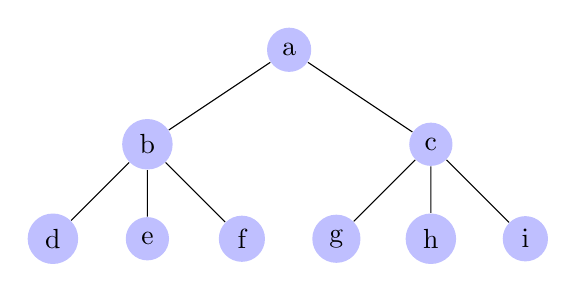
\begin{tikzpicture}
[scale=.8,auto=left,every node/.style={circle,fill=blue!25}]
  \node {a}
  	child{node{b}
  		child{node{d}}
  		child{node{e}}
  		child{node{f}}}
  	child[missing]
  	child[missing]
  	child{node{c}
  		child{node{g}}
  		child{node{h}}
  		child{node{i}}};
\end{tikzpicture}
\caption{Et rodfæstet træ.} 
\label{eksempel_rootedtree}
\end{figure}

\begin{figure}[h]
\centering
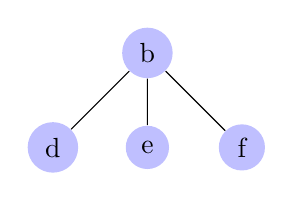
\begin{tikzpicture}
[scale=.8,auto=left,every node/.style={circle,fill=blue!25}]
  \node {b}
  	child{node{d}}
  	child{node{e}}
  	child{node{f}};
\end{tikzpicture}
\caption{Et undertræ med $b$ som rod.} 
\label{eksempel_rootedsubtree}
\end{figure}


\section{Udspændende træer}

Et udspændende træ er et træ, der indeholder alle knuder i en simpel, sammenhængende graf.

\begin{defn}
I en simpel graf $G$ er et udspændende træ en delgraf af $G$, der indeholder alle knuder i $G$, og som også er et træ.
\end{defn}

\noindent En simpel graf med et udspændende træ er sammenhængende, fordi der er vej mellem alle knuder i det udspændende træ. Det omvendte gælder også dvs. at hver simpel sammenhængende graf har et udspændende træ, hvilket kan formuleres i det følgende.

\begin{thm}
En simpel graf er sammenhængende hvis og kun hvis, den har et udspændende træ.
\end{thm}

\begin{proof}
Først antages det, at en simpel graf $G$ har et udspændende træ. 
Træet $T$ vil indeholde alle knuder i $G$ og have en simpel vej mellem alle knudepar, fordi $T$ er et træ. 
Fordi $T$ er den delgraf af $G$, så er der en vej mellem alle knuder i $G$, og derfor er $G$ sammenhængende.

Det antages nu, at $G$ er sammenhængende. Hvis $G$ ikke er et træ, så indeholder den en simpel kreds. 
Der fjernes nu en kant i en af de simple kredse. 
Resultatet er en delgraf af $G$, der har en kant mindre end $G$, og som stadig indeholder alle knuder i $G$ og stadig er sammenhængende. 
Grafen er stadig sammenhængende, fordi knuderne, der var forbunde af den fjernede kant, stadig er forbundne af en vej, der ikke indeholder den fjernede kant, fordi den fjernede kant var en del af en simpel kreds. 
Er der flere simple kredse, gentages processen med at fjerne kanter for at eliminere simple kredse, indtil der ikke er flere. 
Resultatet er et træ, fordi $G$ forbliver sammenhængende, i takt med kanter fjernes. Træet er et udspændende træ, fordi det stadig indeholder alle knuder i $G$.
\end{proof}

\begin{exmp}
Betragt grafgen i Figur \ref{eksempel_udspaendende}. Grafen er simpel og sammenhængende, og derfor kan der findes et udspændende træ. 
\end{exmp}

\begin{figure}[h]
\centering
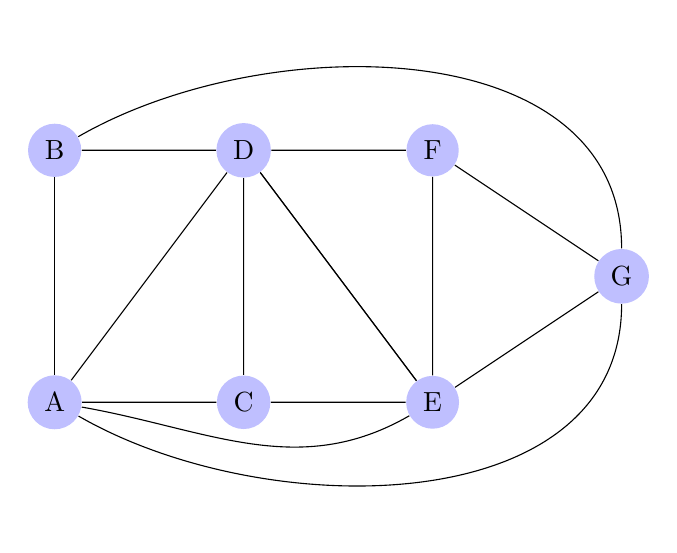
\begin{tikzpicture}
[scale=.8,auto=left,every node/.style={circle,fill=blue!25}]
  \node (n6) at (3,2) {A};
  \node (n4) at (3,6) {B};
  \node (n5) at (6,2) {C};
  \node (n1) at (6,6) {D};
  \node (n2) at (9,2) {E};
  \node (n3) at (9,6) {F};
  \node (n7) at (12,4) {G};
  \foreach \from/\to in {n6/n4,n5/n1,n2/n3,n4/n1,n6/n1,n1/n2,n3/n7,n7/n2,n5/n6,n5/n2,n1/n2,n1/n3}
    \draw (\from) -- (\to);
    \draw (n4) to[out=30,in=90] (n7);
    \draw (n6) to[out=-10,in=-150] (n2);
    \draw (n6) to[out=-30,in=-90] (n7);
\end{tikzpicture}
\caption{En simpel sammenhængende graf} 
\label{eksempel_udspaendende}
\end{figure}

\noindent Der er mange muligheder for at finde et udspændende træ i grafen i Figur \ref{eksempel_udspaendende}. For at finde et udspændende træ, fjernes kanter i de simple kredse, indtil der opstår en sammenhængende undergraf, der indeholder alle knuderne i grafen. To eksempler på udspændende træer ses i Figur \ref{eksempel_udspaendende1} og Figur \ref{eksempel_udspaendende2}.

%Billede med 4 udspændende træer
\begin{figure}[!htb]
\begin{minipage}{1\linewidth}

\centering
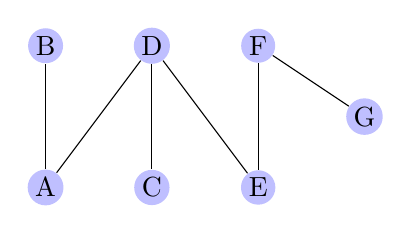
\begin{tikzpicture}
[scale=.45,auto=left,every node/.style={circle,fill=blue!25},inner sep=1pt,minimum size=2pt]
  \node (n6) at (3,2) {A};
  \node (n4) at (3,6) {B};
  \node (n5) at (6,2) {C};
  \node (n1) at (6,6) {D};
  \node (n2) at (9,2) {E};
  \node (n3) at (9,6) {F};
  \node (n7) at (12,4) {G};
  \foreach \from/\to in {n6/n4,n6/n1,n1/n5,n1/n2,n2/n3,n3/n7}
    \draw (\from) -- (\to);
\end{tikzpicture}
\caption{Eksempel på udspændende træ.}
\label{eksempel_udspaendende1}
\end{minipage}

\hfill

\begin{minipage}{1\linewidth}
\centering
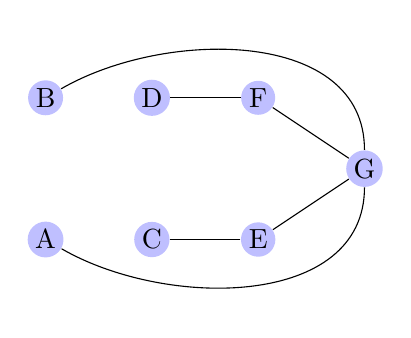
\begin{tikzpicture}
[scale=.45,auto=left,every node/.style={circle,fill=blue!25},inner sep=1pt,minimum size=2pt]
  \node (n6) at (3,2) {A};
  \node (n4) at (3,6) {B};
  \node (n5) at (6,2) {C};
  \node (n1) at (6,6) {D};
  \node (n2) at (9,2) {E};
  \node (n3) at (9,6) {F};
  \node (n7) at (12,4) {G};
  \foreach \from/\to in {n7/n3,n1/n3,n2/n5,n2/n7}
    \draw (\from) -- (\to);
    \draw (n4) to[out=30,in=90] (n7);
	\draw (n6) to[out=-30,in=-90] (n7);
\end{tikzpicture}
 \caption{Eksempel på udspændende træ.}
\label{eksempel_udspaendende2}
\end{minipage}

\end{figure}

\section{Minimum udspændende træer}

En række problemer involverer at finde den eksempelvis korteste, billigste eller på anden vis mest favorable forbindelse, der inkluderer alle knuder i en vægtet graf. Problemet kan løses ved at bestemme et minimum udspændende træ. I et minimum udspændende træ er summen af kanternes vægt er mindst muligt, og træet indeholder alle knuder i grafen.

\begin{defn}
Et minimum udspændende træ i en sammenhængende vægtet graf er et udspændende træ, som har den mindst mulige sum af kanternes vægt.
\end{defn}